\chapter{Introduction}

\section{Background}

\hspace{10mm}
In an era dominated by unprecedented volumes of digital data and an ever-expanding threat landscape, the imperative to secure sensitive information has never been more critical. Traditional encryption methods, while effective in many scenarios, often fall short when it comes to managing access to data in complex, dynamic environments. In response to these challenges, Attribute-Based Encryption (ABE) emerges as a revolutionary paradigm, offering a nuanced and flexible approach to data protection.

ABE represents a departure from conventional encryption models by enabling access control based on attributes rather than traditional cryptographic keys or passwords. This innovative cryptographic technique provides a granular and adaptive means of securing information, aligning more closely with the intricacies of modern data-sharing scenarios. There are several algorithms for ABE like KP-ABE and CP-ABE.

In several distributed systems a user should only be able to access data if a user possesses a certain set of credentials or attributes. Currently, the only method for enforcing such policies is to employ a trusted server to store the data and mediate access control. However, if any server storing the data is compromised, then the confidentiality of the data will be compromised. Ciphertext-policy attribute-based encryption presents a system for realizing complex access control on encrypted data that we call. By using these techniques encrypted data can be kept confidential even if the storage server is untrusted; moreover, these methods are secure against collusion attacks. Previous attribute-based encryption systems used attributes to describe the encrypted data and built policies into user's keys; while in the system attributes are used to describe a user's credentials, and a party encrypting data determines a policy for who can decrypt. Thus, these methods are conceptually closer to traditional access control methods such as role-based access control .
Ciphertext-policy attribute-based encryption (CP-ABE) to address this problem, and give the first construction of such a scheme. In the system,a user’s private key will be associated with an arbitrary number of attributes expressed as strings. On the other hand, when a party encrypts a message in our system, they specify an associated access structure over attributes. A user will only be able to decrypt a ciphertext if that user’s attributes pass through the ciphetext’s access structure. At a mathematical level, access structures in our system are described by a monotonic “access tree”, where nodes of the access structure are composed of threshold gates and the leave describe attributes. We note that AND gates can be constructed as n-of-n threshold gates and OR gates as 1-of-n threshold gates. Furthermore, we can handle more complex access controls such as numeric ranges by converting them to small access trees 
\section{Encryption}
The process of converting the original representation of the information, known as plaintext into an alternative form known as cipher-text. Modern encryption schemes use the concepts of public-key and symmetric-key. 
In symmetric-key schemes, the encryption and decryption keys are the same. Communicating parties must have the same key in order to achieve secure communication. In public-key encryption schemes, the encryption key is published for anyone to use and encrypt messages. However, only the receiving party has access to the decryption key that enables messages to be read. 
           
\section{Fine-grained Access Control}
Fine-grained access control systems facilitate granting differential access rights to a set of users and allow flexibility in specifying the access rights of individual users. Identity-Based Encryption (IBE) is a cryptographic scheme that is related to the concepts of fine-grained access control.

\section{Identity Based Encryption}
Identity based encryption is a type of public-key encryption in which the public key of a user is some unique information about the identity of the user (e.g. a user's email address). This means that a sender who has access to the public parameters of the system can encrypt a message. The receiver obtains its decryption key from a central authority, which needs to be trusted as it generates secret keys for every user. 

\begin{figure}[h]
    \centering
   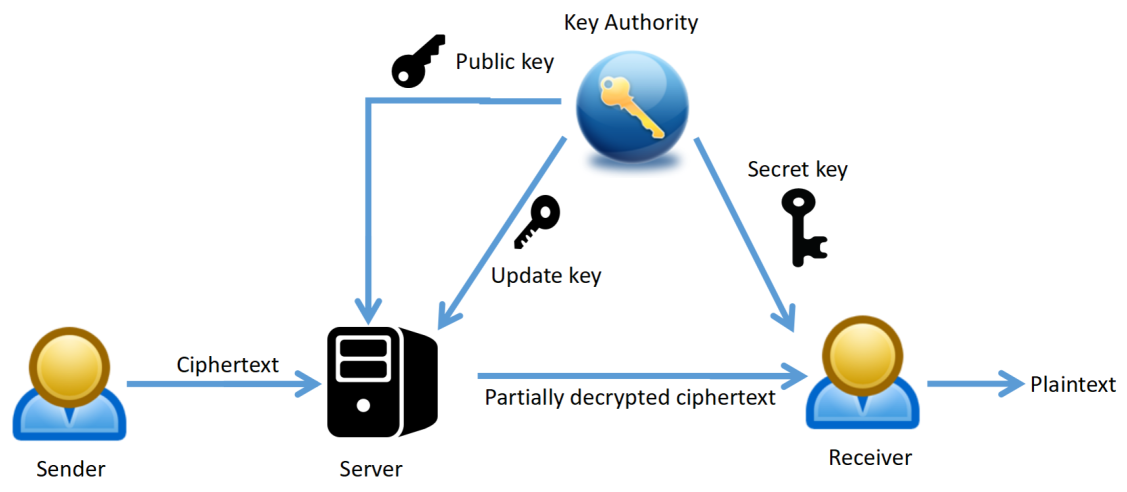
\includegraphics[width=\linewidth]{Images/IBEV2.png}
    \caption{Example of Identity Based Encryption}
    \label{fig:enter-label}
\end{figure}

\section{Attribute Based Encryption}
Attribute-based encryption is probably a generalization of identity-based encryption which enables fine grained access control of encrypted data using authorisation policies. The secret key of a user and the ciphertext are dependent upon attributes (e.g. their email address, the country in which they live, or the kind of subscription they have). In such a system, the decryption of a ciphertext is possible only if the set of attributes of the user key matches the attributes of the ciphertext.Researchers have further proposed attribute-based encryption with multiple authorities who jointly generate users' private keys. There are mainly two types of attribute-based encryption schemes: Key-policy attribute-based encryption (KP-ABE) and ciphertext-policy attribute-based encryption (CP-ABE).
An important property which has to be achieved by both, CP-ABE and KP-ABE is called collusion resistance. If multiple users try to access the encrypted data, they should only be able to decrypt a ciphertext if at least one of the users could decrypt it on their own. Both CP-ABE and KP-ABE provide Collusion Resistance.
\section{Access Policies}
Access policies refer to rules that govern the permissions and restrictions placed on entities attempting to access cryptographic resources. Here are some types of access policies commonly used:
\begin{itemize}

    \item\bm AND-Gate Policy: This policy requires that a user possesses all specified attributes for access.

    \item\bm OR-Gate Policy: An OR-Gate policy allows access if a user possesses at least one of the specified attributes.

\end{itemize}
\begin{figure}
    \centering
   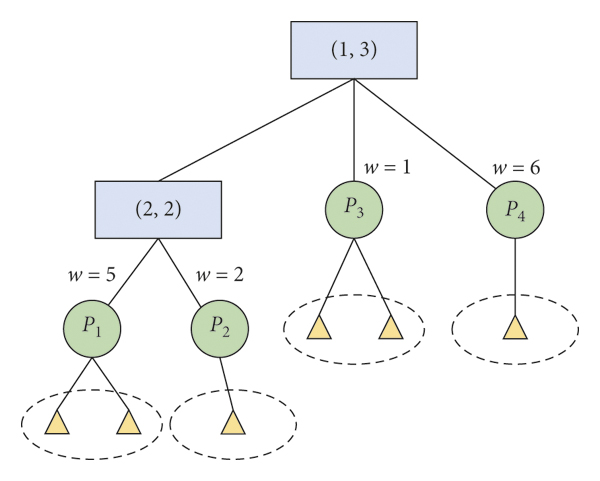
\includegraphics[width=\linewidth]{Images/ABE.png}
    \caption{Example of Attribute Based Encryption}
    \label{fig:enter-label}
\end{figure}
\begin{figure}
    \centering
   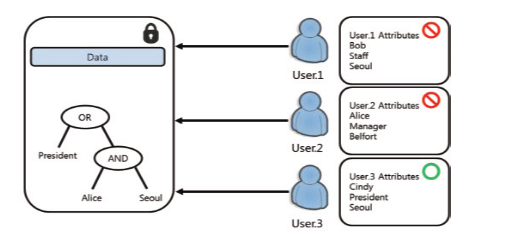
\includegraphics[width=\linewidth]{Images/ANDOR.png}
    \caption{Example of Attribute Based Encryption}
    \label{fig:enter-label}
\end{figure}